To add a second chapter, simply include it in the main document.

\section{General structure}
\subsection{JModelica(Compile)Phase}
The JModelica environment is used to compile the Modelica models to JModelicas JMU representation \cite{jmodelicaorg}\nocite{*}. This representation is internally represented as a, possibly nonlinear, DAE. Since ProMoVis assumes the systems to be linear, the compiled model needs to be linearised around an operating point. Here an assumption is made, that the model is stable at Time 0. See Appendix \ref{appA} for a complete overview of the prerequisites for the original model.\\\\After linearisation a DAE on the following form can be extracted:
\begin{equation}
E*dx = A*x + B*u + F*w + g
\end{equation}
This represenation should be familiar, the x and dx vectors represents the states and outputs of the linearized system. The u vector represents declared inputs, w is algebraic varibles, that is all variables in the system that has no derivative declared.Finally g is a constant bias.\\\\The linearization also outputs some useful information that we later use in the generation of ProMoVis scenarios:
\begin{itemize}
\item \textit{State names}, corresponding to the declared variable names from the original Modelica file.
\item \textit{Input names}, corresponding to the declared input names from the original Modelica file.
\item \textit{Algebraic names}, corresponding to the declared algebraic variable names from the original Modelica file.
\item \textit{Operating points} for the linear model \textit{dx0},\textit{w0}, \textit{u0} and \textit{x0}. Which is , in later stages, used to provide feedback for the user regarding the validity of the resulting model.
\end{itemize}
From now on we will refer to states and algebraic variables as simply "variables" and whenever a distinction between the two is needed, it will be explicitly declared. 

\subsection{Generation of the internal structure}
When the DAE is obtained, the task is then to extract the relations between the variables from it. Here we choose to collect and store each of the variables, together with each of the variables that acts as input to it. It might feel more natural to store a variable together with each of its outputvariables but since ProMoVis supports both conventions and due to the fact that it is straight forward to solve a variable for all its inputs from the original DAE the first representation was choosen.
The generation of the internal structure is best illustrated with the following example.\\\newline
If we assume two state variables and two algebraic variables, the general structure of the DAE would look like the following:\\\newline
$
\begin{bmatrix} E_{11} & E_{12} \\ E_{21} & E_{22} \\ E_{31} & E_{32} \\ E_{41} & E_{42} \end{bmatrix} \left[ \begin{array}{c} x0' \\ x1' \end{array} \right]
= \begin{bmatrix} A_{11} & A_{12} \\ A_{21} & A_{22} \\ A_{31} & A_{32} \\ A_{41} & A_{42} \end{bmatrix} \times \left[ \begin{array}{c} x0 \\ x1 \end{array} \right] + \begin{bmatrix} B_{11} & B_{12} \\ B_{21} & B_{22} \\ B_{31} & B_{32} \\ B_{41} & B_{42} \end{bmatrix} \times \left[ \begin{array}{c} u0 \\ u1 \end{array} \right]+
\begin{bmatrix} F_{11} & F_{12} \\ F_{21} & F_{22} \\ F_{31} & F_{32} \\ F_{41} & F_{42}\end{bmatrix} \times \left[ \begin{array}{c} w0 \\ w1 \end{array} \right]$

The task is now, to find which of the rows in the system that should be solved for which variable so that the whole system can be solved. A demand on the system is that it should not contain any Algebraic loops. For a more thorough discussion regarding this please review Appendix \ref{appB}\\\\After retrieving which row that we should solve for which of the variables we build up an intermediate representation of the SFG where we store each of the variables together with all of its input variables.\\\\
As an example, if we assume that we should solve row 1 for x0 the procedure is as follows:\\\\$\begin{array}{rcl} E_{11}*x0*s  +E_{12}*x1*s=A_{11}*x0  +A_{12}*x1 +B_{11}*u0  +B_{12}*u1  +F_{11}*w0  +F_{12}*w1 \end{array}$\\
\\Putting x0 alone on the left-hand side and collecting the coefficients then yields:\\\\$\begin{array}{rcl} (E_{11}*s-A_{11})*x0  =(A_{12}-E_{12}*s)*x1 +B_{11}*u0  +B_{12}*u1 +F_{11}*w0  +F_{12}*w1 \end{array}$\\\\
Finally, solving for x0 yields:\\\\
$\begin{array}{rcl} x0  = \frac{(A_{12}-E_{12}*s)}{(E_{11}*s-A_{11})}*x1 +\frac{B_{11}}{(E_{11}*s-A_{11})}*u0  +\frac{B_{12}}{(E_{11}*s-A_{11})}*u1 ++\frac{F_{11}}{(E_{11}*s-A_{11})}*w0 +\frac{F_{12}}{(E_{11}*s-A_{11})}*w1\end{array}$\\\newline Which would correspond to the following SFG:\\Internally we then represent each of the variables in the following form.\\\newline
%

\setlength\fboxsep{0pt}
\setlength\fboxrule{0.5pt}
\fbox{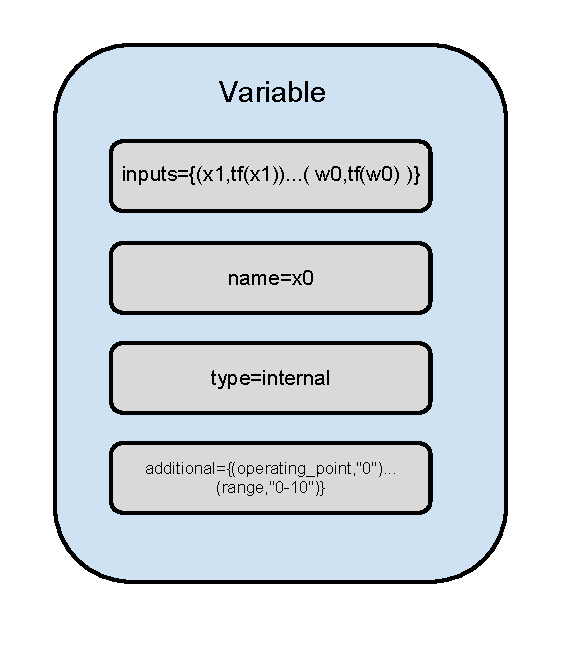
\includegraphics[scale=0.8,bb=0 0 97mm 111mm] {Figures/variable_structure.pdf}}\\\newline Here "inputs" is a dictionary with variable names as keys and the corresponding transfer functions as a values. A transfer function, in the export tool,is using the same convention as in MatLab to represent the numerator and denominator coefficients for a transfer function in two separate arrays. It also has some methods, described later, that are used in the generations of the ProMoVis specific structure. 


\subsection{Validation and Transformations}
\subsection{Scenario generation}
When the structure is validated and all optional transformations are done. The actual generation of the ProMoVis represenation is straight forward. Basically the ProMoVis representation contains two parts. First the descriptive part, a collection of all variables, with their names, graphical layout and additional mathematical properties. The second part,  the processmodels, describes the relation between a variable and the other variables in the system. 
\subsubsection{Graphical Layout}
Even though Modelica supports description of position and graphical represenation of models through its annotations interface, these are not necessary for a valid Modelica model. Therefore no effort has been put into trying to recieve this type of meta-information. Instead, to make sure that a user of ProMoVis is able to easilly access and attach controllers to the generated model the variables are emitted as depicted in the figure below.\\\newline
\setlength\fboxsep{0pt}
\setlength\fboxrule{0.5pt}
\fbox{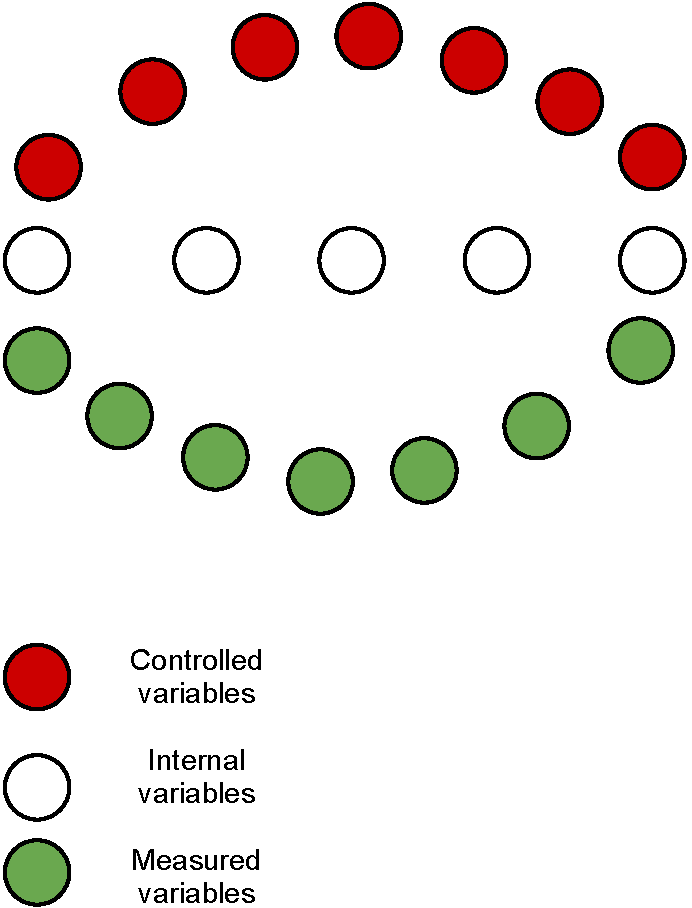
\includegraphics[scale=0.8,bb=0 0 117mm 154mm] {Figures/layout.pdf}}\\\newline

That is, inputs and measured variables are emitted as the upper and lower half of a circle while internal variables, that are assumed to not be of interest, are collected in the center of the circle. This achieved by a helper object, the layout emitter, that is initiated with the number of internal, measured and input variables and then calculates the step size in x and y direction that will eventually achieve the circular shape. 

When we then iterate over each of the variables to get their corresponding descriptive part, the layout emitter is passed as an argument, so that it can be queried for the variables graphical x and y position. This i done in a very naive way, the layout emitter has counters for each of the variable types and then, each time it is queried, it increments the current counter value together with the previously calculated step sizes to generate one x,y coordinate that is returned to the querying variable. 
\subsubsection{Additional information added}

\section{Interfacing with the tool}
Since there are several seperate phases in the tool, and each of the phases might later be extended with additional options and necessary parameters xml is used to pass information to the tool. By using xml and not command line arguments one might, through using existing modules for xml-parsing and object representation of the xml files, just pass the instance of the "parsed" xml document to each of the phases. Where they then might extract the information needed for the phases.FIXME\\\\Following is an example of the input file to the tool, containing all the necessary parameters.
\begin{lstlisting}
<?xml version="1.0" ?> 
<root>
        <filepath>C:\Users\Public\Documents\QuadTankPack.mo</filepath>
        <model>QuadTankPack.QuadTank</model>
        <mpattern>_pmv;_fooBar;x2</mpattern>
        <outputpath>C:\ProMoVis\output.xml</outputpath>
        <pmvoutputpath>C:\ProMoVis\QuadTank.pmv</pmvoutputpath>
</root>
\end{lstlisting}
The filepath and model nodes are the path to the original modelica source file and the full model name, including packagenames, of the target model. The node, mpattern, contains regular expression that the tool will try to match the ending of variable names on, so that if it encounters the variables foo\_pmv, foo\_foobar, foox2 or x2 it will make sure that those variables are indicated as measured variables in the ProMoVis representation.


\section{DAE vs ODE}
Readers familiar with Modelica and the JModelica environment might be accustomed to working on the ODE-representation of systems. The reason that we stick with the DAE even though the extraction of the SFG from the ODE is less complex is due to the fact that when using the ODE we loose casuality whenever an algebraic variable is in a path. Recall the general DAE representation:
\begin{equation}
E*dx = A*x + B*u + F*w + g
\end{equation}

Introducing the ODE representation that also can be extracted:

\begin{equation}
dx = A*x + B*u + g
\end{equation}
\begin{equation}
w  = H*x + M*u + q
\end{equation}

Here it might be tempting to create the SFGs from the ODE instead, since one can solve for the states and algebraic variables separately. But notice, now the states does not depend at all on the algebraic variables in w. This is still a correct system, since algebraic variables is only a combination of other states, algebraic variables and constants thus they can be reduced and replaced by other states and a constant. But even though it is mathematically correct, we have lost information. The casuality is broken, and a user that has declared states that depends on algebraic variables can no longer view and analyse such a relation inside ProMoVis. One can easilly see this by just looking at the ODE and DAE representations above, the algebraic variables in w only has inputs and never acts as an input itself and therefore will become leafs in the SFG. FIXME DO WE NEED APPENDIX EXPLAINING THIS MORE THOROUGHLY.
\section{A small case study}